\section{Solução}

A análise das principais ferramentas disponíveis para gerenciamento de \textit{workflow} indicou o \textit{Airflow} como mais adequada ao contexto do TRE-RN. A adoção do \textit{Airflow} requer algumas decisões de projeto, como a arquitetura a ser adotada e a implantação dessa solução. Nesta seção, discutimos inicialmente as opções de arquitetura disponibilizadas pelo \textit{Airflow}, detalhando a que propomos para o TRE-RN. Em seguida, relatamos a implantação realizada, avaliando a solução proposta a partir de um conjunto real de \textit{workflows} de ETL já utilizados no tribunal.

% A partir das ferramentas apresentadas, através de uma análise de usabilidade definimos o Airflow  como a ferramenta que melhor se atende as necessidades através dos seguintes critérios.

% Com base na análise das ferramentas, decidimos qual a ferramenta que melhor se adapta ao contexto do TRE-RN e com base nessa ferramenta, decidimos um arquitetura que pudesse atender as necessidades do TRE-RN e que fosse viável.

\subsection{Arquitetura}

O \textit{Airflow} oferece dois tipos de arquiteturas, diferentes em função do número de nós (\textit{workers}) utilizados. A Figura~\ref{fig:airflow-architecture} ilustra todos os componentes comum a ambas arquiteturas disponíveis no \textit{Airflow}. A diferença entre o modelo com um ou múltiplos \textit{workers} está encapsulada no componente \textit{workers}. Os demais componentes são detalhados a seguir:

\begin{figure}[!t]
    \centering
    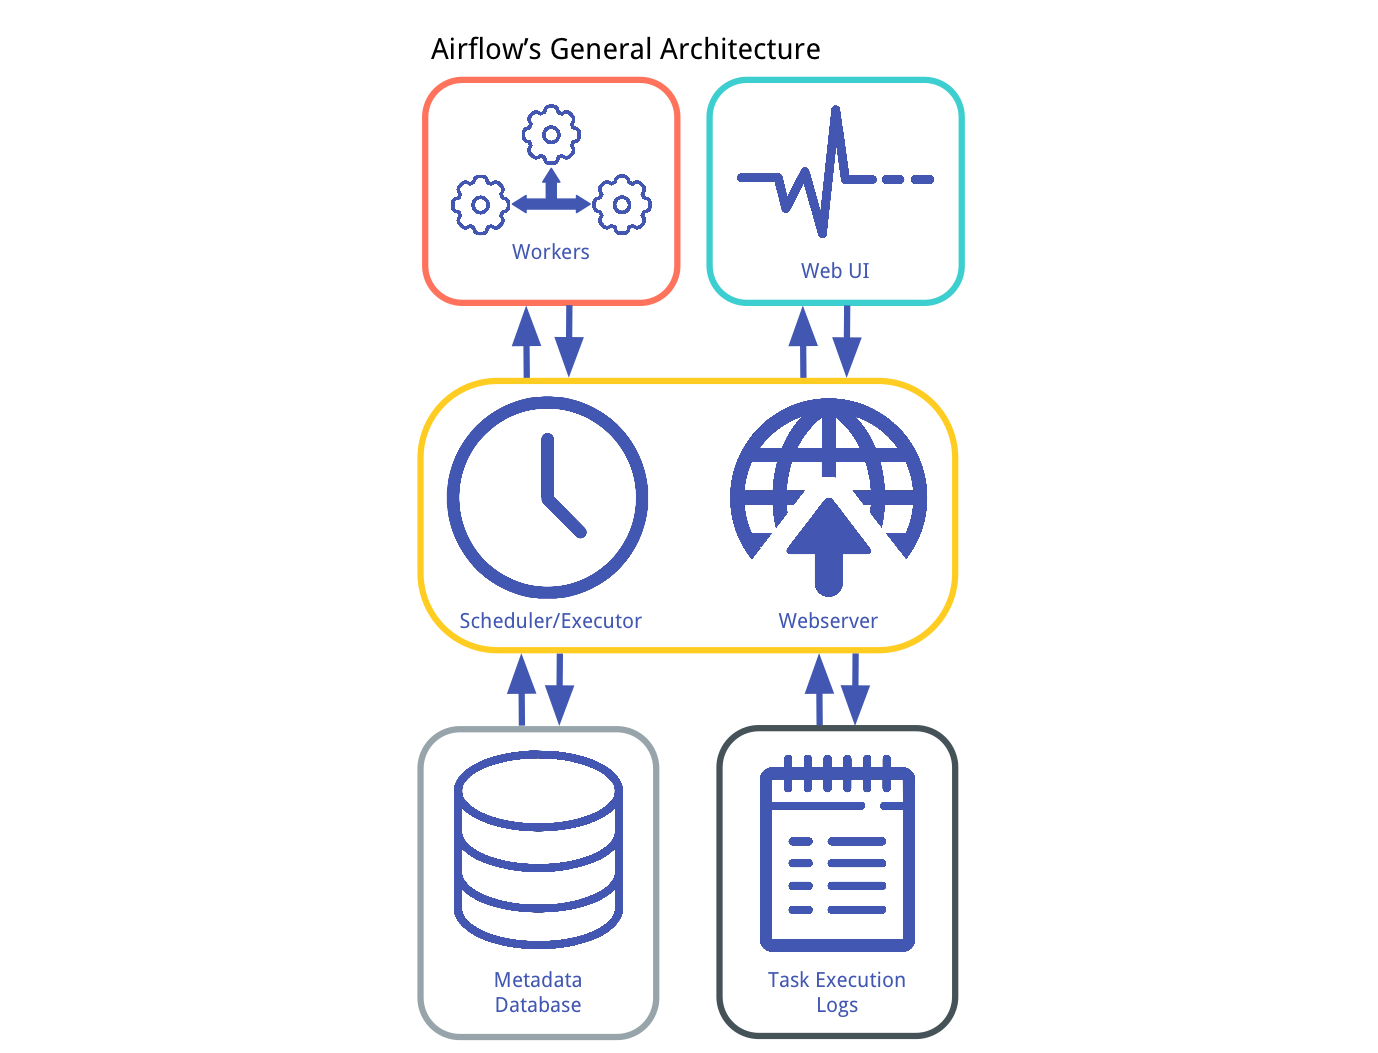
\includegraphics[width=\linewidth]{Imagens/airflow-architecture.png}
    \caption{Arquitetura Airflow}
    \label{fig:airflow-architecture}
\end{figure}

\textbf{Metadata database} - metadados dos \textit{workflows}.

\textbf{Execution logs} - resultados das execuções dos \textit{workflows}.

\textbf{Webserver} - \textit{back-end} da interface gráfica.

\textbf{Web UI} - \textit{front-end} da interface gráfica.

\textbf{Scheduler/Executor} - gerencia a execução dos \textit{workflows}.

Atualmente no TRE-RN, os \textit{workflows} de ETL são executados em um servidor de agendamentos, denominado \textit{pocoyo}, que reúne os agendamentos feitos via CRON. Há também um servidor de aplicação, que reúne as aplicações \textit{web} disponibilizadas pelo tribunal para uso interno e externo. Considerando este contexto, propomos duas arquiteturas para a implantação do \textit{Airflow}:

% A partir da seleção da ferramenta, pensamos em duas arquiteturas usando o Airflow para a contexto no TRE-RN.
\paragraph{\textit{Container} em um único servidor:}
a primeira solução consiste na utilização de um \textit{container Docker} reunindo o \textit{Airflow} e o PDI. Com esta abordagem, todo o processo de ETL estaria concentrado em um único local. Esta abordagem é apresentada na Figura~\ref{fig:docker}.

\begin{figure}[htp]
    \centering
    
\includegraphics[width=3cm]{Imagens/Arq_1}
    \caption{Arquitetura reunindo o \textit{Airflow} e o \textit{PDI} em único \textit{container Docker}.}
    \label{fig:docker}
\end{figure}

Apesar de ser uma solução agregadora, a infraestrutura do TRE-RN inviabiliza esta opção. Especificamente, o servidor \textit{pocoyo} não suporta \textit{containers}, nem há interesse por parte do tribunal de que o servidor seja usado para hospedar um serviço \textit{web} (interface do \textit{Airflow}). Assim, seria necessário hospedar o \textit{container} no servidor de aplicações \textit{web}. No entanto, com esta opção os sistemas existentes teriam perda de performance, devido ao consumo elevado de recursos por parte do PDI. 

\paragraph{\textit{Pocoyo} como \textit{worker} remoto:}
na segunda proposta de arquitetura, ilustrada na Figura~\ref{fig:ssh}, desacoplamos o PDI do \textit{container} que contém o Airflow. Efetivamente, o \textit{Airflow} seria hospedado no servidor de aplicações \textit{web}, enquanto o processo de ETL continuaria a ser executado no servidor de agendamento \textit{pocoyo}. Por esta arquitetura, o \textit{Airflow} enxerga o \textit{pocoyo} como um \textit{worker} remoto, com a comunicação sendo feita pelo protocolo SSH (\textit{secure shell},~\citet{}). Desse modo, o consumo de recursos no servidor de aplicação seria reduzido, utilizando o \textit{Airflow} apenas como um interface para a execução remota dos \textit{workflows}. 

\begin{figure}[htp]
    \centering
    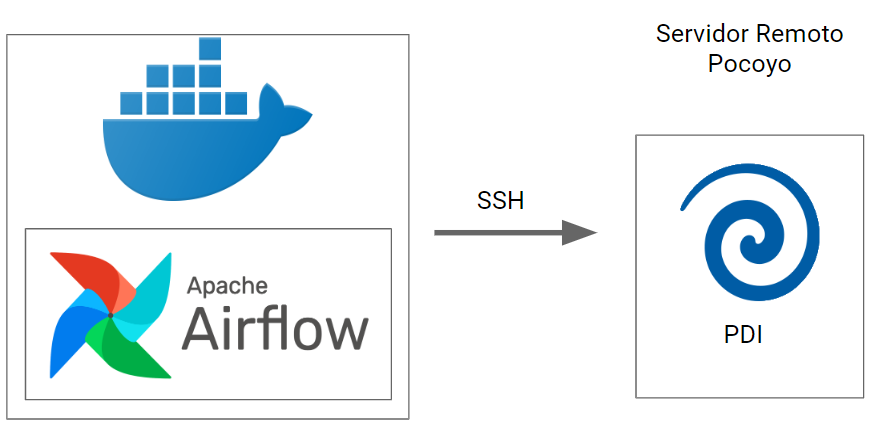
\includegraphics[width=8cm]{Imagens/Arq_2}
    \caption{Arquitetura usando o \textit{pocoyo} como \textit{worker} remoto.}
    \label{fig:ssh}
\end{figure}

\subsection{Implantação}

Com a implantação da arquitetura, criamos jobs usando Airflow para fazermos o mesmo processo que é feito atualmente com Cron. Usando alguns exemplos, conseguimos observar o resultado de como seria a aplicação em um cenário mais próximo de produção. Como resultado, observamos que o gerenciamento dos ETL’s ficou mais simples, devido a interface gráfica.


\begin{figure*}[htp]
    \centering
    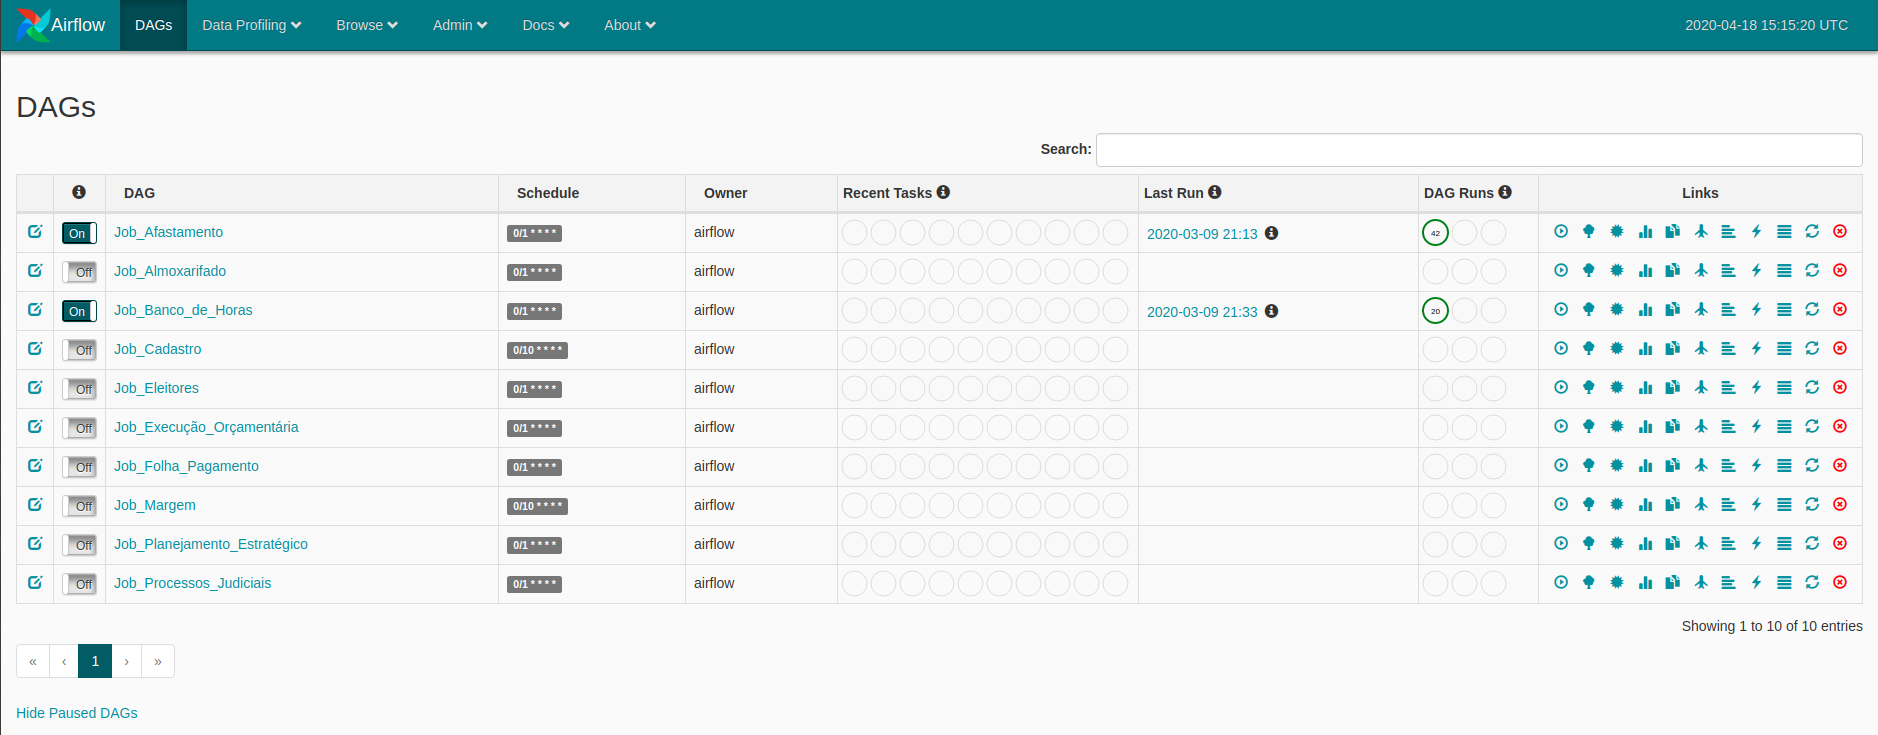
\includegraphics[width=\linewidth]{Imagens/Airflow_End}
    \caption{Airflow com Jobs do TRE}
    \label{fig:airflow-tre}
\end{figure*}
